\chapter{Results and Analysis}
\label{details}
After introducing the basic knowledge which is available and used in the project, I will start the experiments and analyze the results. The main experiments would be,
\begin{enumerate}
    \item Do the simulation based one computer physics library(\textit{pybox2d}). Totally, 100 different rigid motion simulation would be carried out. For every simulation, I would record the fixed number of simulation steps, $600$.
    \item \textbf{XML} formulation would be used to store every step of all simulation. The data of each state would involve positions, velocities, contact forces, etc.
    \item Once obtaining the \textbf{XML} files. I would transform the \textbf{XML} files into a \textit{pybox2d} world, and then carry out some experiments to determine different grid size and smoothing length of SPH.
    \item After choosing the proper parameter of the SPH kernel(types, grid cell size, and smoothing length), I would transform these \textbf{XML} files to grid images, which are used as training dataset. 
    \item Design a deep learning model and do the training on the training dataset.
    \item Apply the trained model to predict the starting iterate values of contact forces($\pmb{\lambda}$). Then I would compare the learning model with other classical methods.
\end{enumerate}

\section{Rigid Motion Simulation}

\textit{pybox2d}\footnote{\url{https://github.com/pybox2d/pybox2d}} is chosen as the main physics engine to implement computer simulation experiments. \textit{pybox2d} is a 2D physics library for your games and simple simulations. It's based on the Box2D library, which is written in \textit{C++}. It supports several shape types (circle, polygon, thin line segments), and quite a few joint types (revolute, prismatic, wheel, etc.). In my experiment, I would first try to apply deep learning in the simple simulations. So I would mainly simulation with circle rigid objects sharing the same radius. 

\subsection{Simulation Configuration}
Simulation configs are listed below,
    \label{simconfig}
    \begin{itemize}
        \item \textbf{World Setting}, the world box size is $30\times30$,   and there are $100$ circle rigids($r=1$, all circle rigid bodies in the same size.) inside the box. Initially, the rigid circles will be located following gaussian distribution\footnote{\url{https://en.wikipedia.org/wiki/Normal_distribution}}. Then, all rigid circles will fall down by gravity. The visualization of simulation is shown in Figure \ref{fig:imsim}.
        \item \textbf{Simulation Setting}, there will be totally $600$-steps simulation. For each step, $\Delta t = 0.01s$, and the number of iteration in each step will be set as fixed, $3000$. Then I will use the average convergence rate to describe the performances of models.
    \end{itemize}
\subsection{Simulation Details}
    Before generating data, one dynamic simulation was run to check how \textit{pybox2d} works and some figures have been obtained. Figure \ref{fig:contactnum} describe the relationship between time step and contacts number, and Figure \ref{fig:contacttime} gives the relationship between time spend and contacts number.
    \begin{figure}[!h]
        \centering
        \begin{subfigure}[b]{0.3\textwidth}
            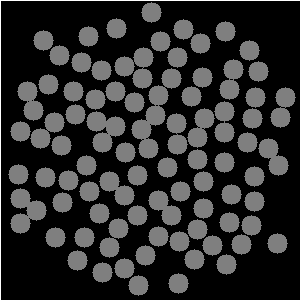
\includegraphics[width=\textwidth]{Figures/sim0.png}
            \caption{Time Step=$0$}
        \end{subfigure}
        \begin{subfigure}[b]{0.3\textwidth}
            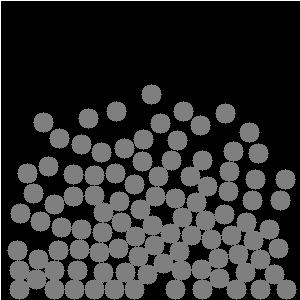
\includegraphics[width=\textwidth]{Figures/sim2.png}
            \caption{Time Step=$200$}
        \end{subfigure}
        \begin{subfigure}[b]{0.3\textwidth}
            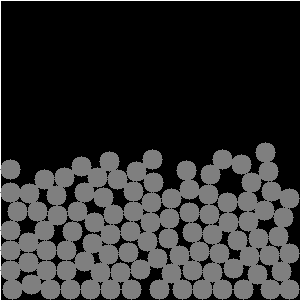
\includegraphics[width=\textwidth]{Figures/sim3.png}
            \caption{Time Step=$400$}
        \end{subfigure}
        \caption{Visualization for experiment simulation}
        \label{fig:imsim}
    \end{figure}
    \begin{figure}[!ht]
        \centering
        \begin{subfigure}[b]{0.7\textwidth}
            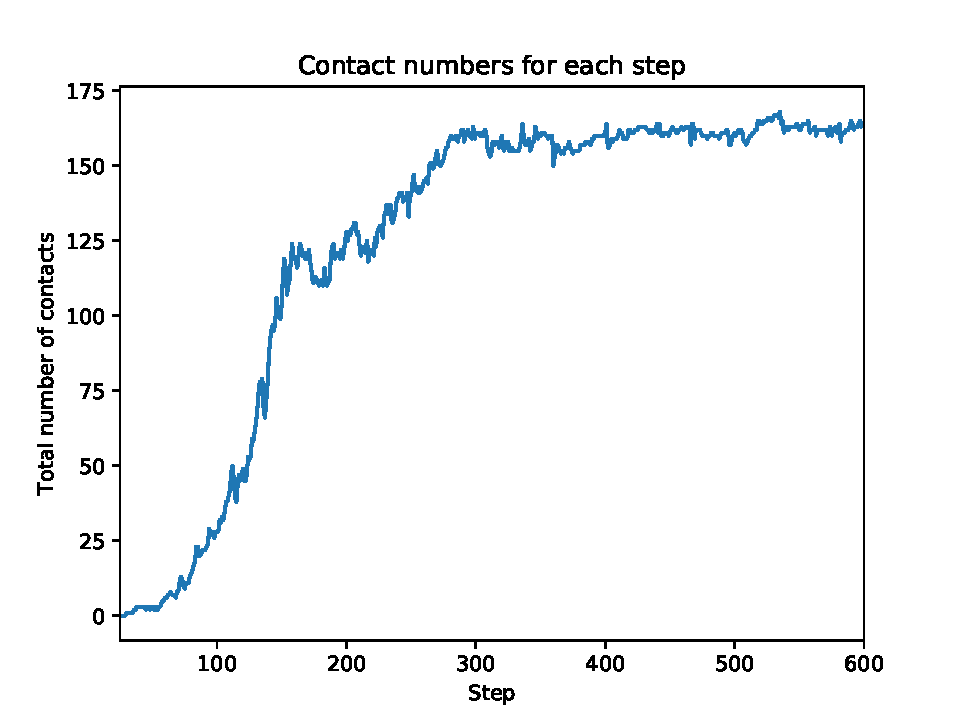
\includegraphics[width=\textwidth]{Figures/contact_num}
            \caption{The number of contacts in each step.}
            \label{fig:contactnum}
        \end{subfigure}
        \begin{subfigure}[b]{0.7\textwidth}
            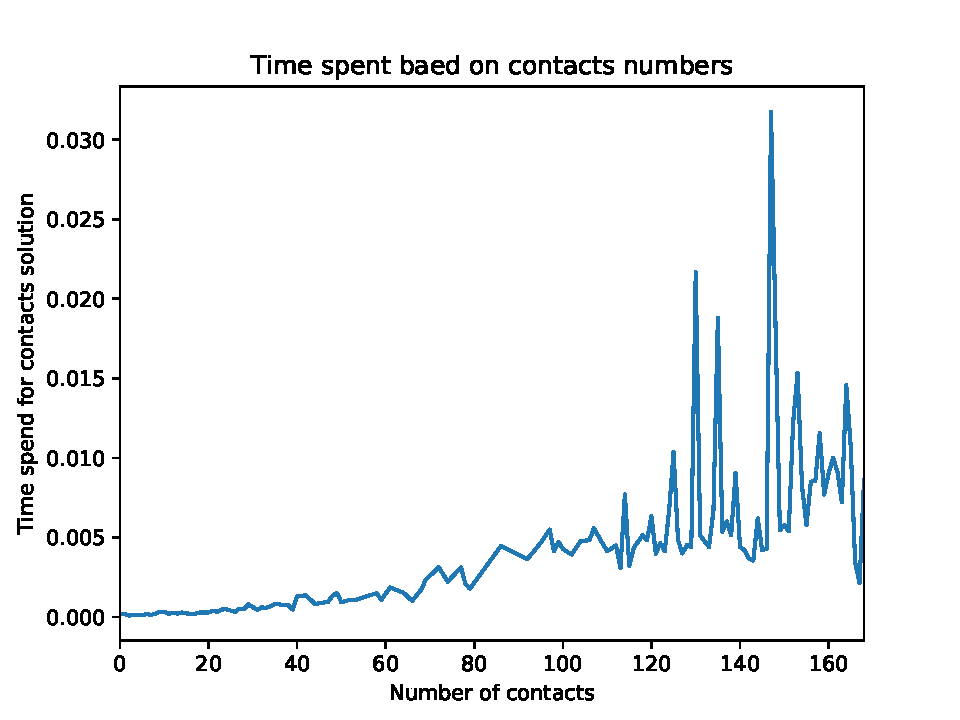
\includegraphics[width=\textwidth]{Figures/contact_time}
            \caption{Time spent for contact solutions.}
            \label{fig:contacttime}
        \end{subfigure}
        \caption{Visualization for experiment simulation}
    \end{figure}

\subsection{SPH parameters}
    \label{SPH-setting}
    In Section \ref{sphtest}, it has been tested that \textbf{SPH} is a good strategy to generate grid images representing a discrete snapshot of the dynamics. Then, the grid size and smoothing length $h$ are imported into our data generation. The grid size should be reasonable so that there is no two contact points are mapped into the same cell, since if there are more than two contact values in one cell, the rid node might store mixture information state from two objects. which would be hard for CNN to find the relationship within one objects, which will decrease the accuracy of prediction. This was mentioned in section \ref{gs}.
    \begin{figure}[!h]
        \centering
        \includegraphics[width=0.4\textwidth]{Figures/SPHvi.pdf}
        \caption{Example visiualization for Smoothed Particle Hydrodynamics. The small red circles stand for the grid nodes, and the blue circles stand for kernel size.}
    \end{figure}

    \subsubsection{Grid Size and Kernel Length}
    I define $\pmb{d}=(d_x, d_y)$ as grid cell size and $h$ as smoothing length. I conclude some rules for determining grid cell size and smoothing length. 
    \begin{itemize}
        \item Since the objects are circles, the ideal cell size should like,
            $$d_x = d_y = d $$ 
        \item Since there can not be two contact points are mapped into the same cell, $d$ must be less than the distance of nearest two contact points. It can be defined.
            $$d \le r = 1$$
        \item Similarly, if one contact point can only be mapped to one cell, the smooth length $h$ should be less than the minimum distance between two contact points $d$,
            $$h \le d$$  
        \item For a given $d$, whatever the contact position $\pmb{q}=(q_x, q_y)$ is, its information can be restore in nearby nodes. So it can be,
            $$h \ge \frac{\sqrt{2}}{2}d \approx 0.71 d$$
    \end{itemize}
    One experiment has been designed to test whether the rules can be applied in this case. Still using the simulation config introduced in section \ref{simconfig}. The cell size is fixed, $d=0.25$. Different smoothing length is appiled. The results are shown in Figure \ref{fig:dh}.

    \begin{figure}[!ht]
     \centering
    \begin{subfigure}[b]{0.7\textwidth}
        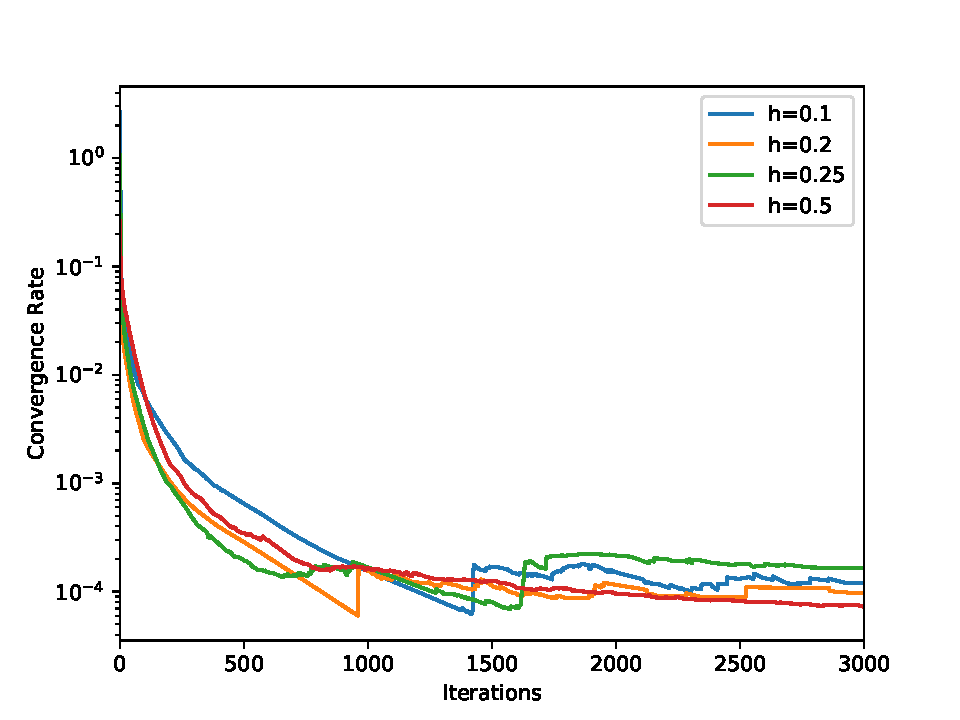
\includegraphics[width=\textwidth]{Figures/size25.pdf}
        \caption{The grid size $d$ is set $0.25$. $h=0.1, 0.2, 0.25, 0.5$ is tested respectively. This figure shows different coveragence rate based on different $h$ value.}
        \label{fig:dh}
    \end{subfigure}
    \begin{subfigure}[b]{0.7\textwidth}
        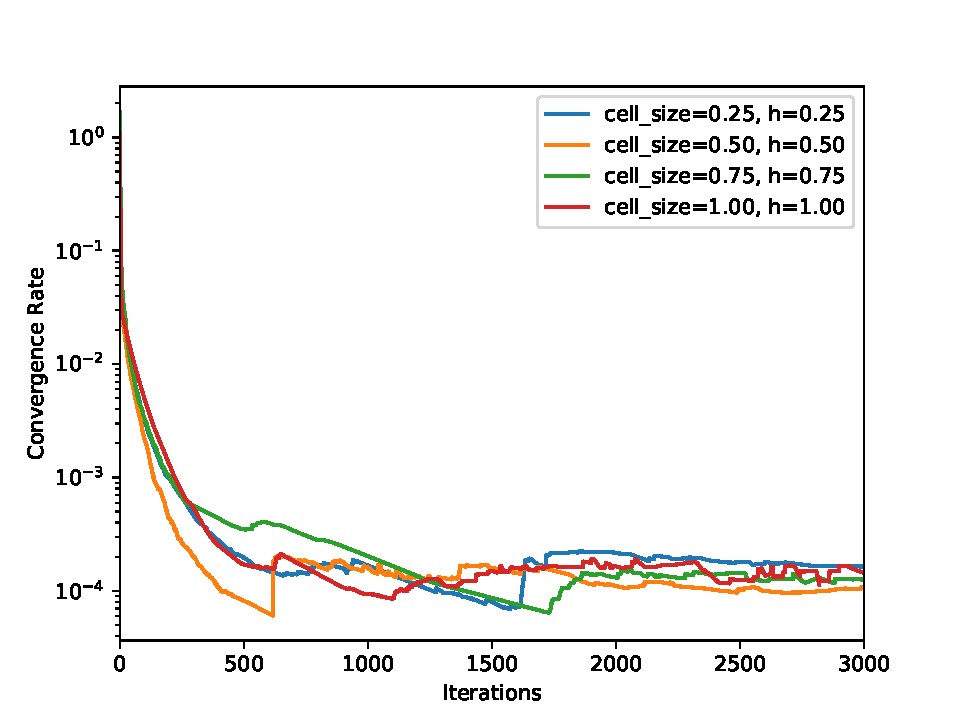
\includegraphics[width=\textwidth]{Figures/hd.pdf}
        \caption{Coveragence rate for different $d$ value.}
        \label{fig:testd}
    \end{subfigure}
    \caption{Experiments from kernel \textbf{Poly6}}
    \label{poly6}
    \end{figure}

    As what is shown in Figure \ref{fig:dh}, when $h=0.4d$ or $h=2d$, the solver coverages more slowly and unstable. Overall, for the next step, data generation, I will make $h=d$ always. The next step is to explore what $d$ value will be good. Once $h=d$ has been determined, the next step is to choose the value of $d$. Another experiment is taken to check the convergence rate with using diffrent $d$ values. The reults are showns in Figure \ref{fig:testd}. From this figure, it is obviously, when $d=0.5$, iterative solver converages the most rapidly. 
    \textbf{Importantly}, $d=0.5~~\text{and}~~h=0.5$ is not always the best experimented with different numbers of rigid inside the world box. But, it generally performs better than other values. As a result, I will choose $h=d=0.5$ as the parameters for SPH method.
    $$d_x = d_y = 0.5~~\text{and}~~h=0.5$$
    \subsubsection{Kernel Choosing}
    The choice of kernel also needs to be addressed. In the paper, two kernels, \textbf{Poly6} and \textbf{Spiky}, have been introduced in section \ref{sec:kernels}. In order to compare these two kernels and determine the best one, finding the best parameters for \textbf{Spiky} is essential. I did the same experiment with kernel \textbf{Spiky}. Find a good scale between $h$ and $d$ firstly and then choose $d$. The results are shown in Figure \ref{spiky}. The plot in Figure \ref{fig:spikynum} reveals that $h=d$ is also a good choice for kernel \textbf{Spiky}. Although $d$s perform similarly, $d=0.25$ performs more stable and a bit fater in convergence. \\
    \begin{figure}[!ht]
        \centering
        \begin{subfigure}[b]{0.7\textwidth}
            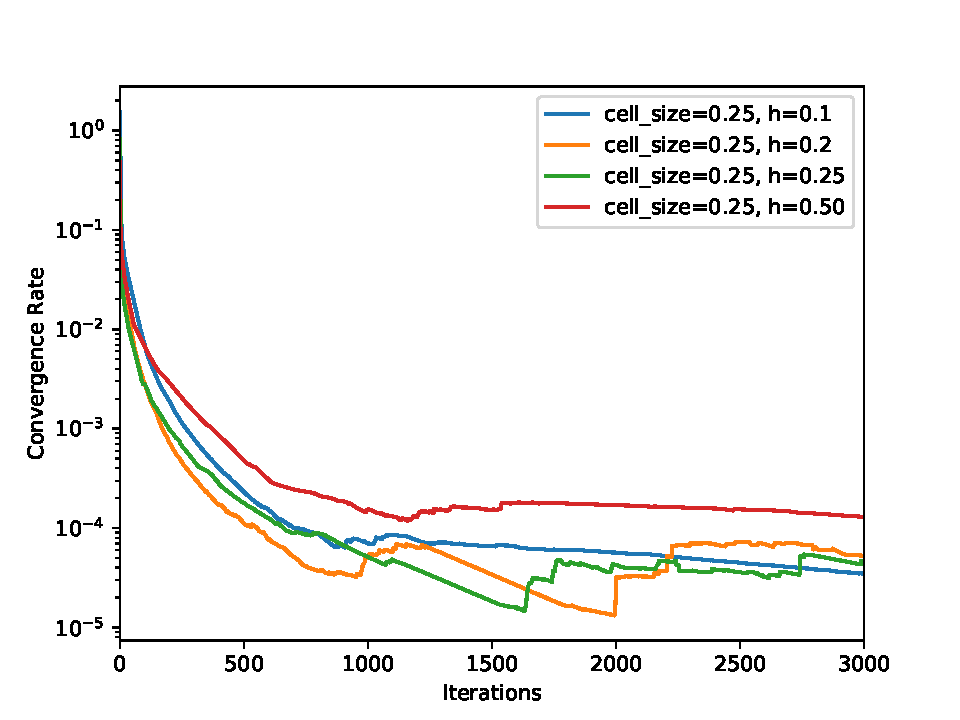
\includegraphics[width=\textwidth]{Figures/spiky25.pdf}
            \caption{The grid size $d$ is set $0.25$. $h=0.1, 0.2, 0.25, 0.5$ is tested respectively. This figure shows different coveragence rate based on different $h$ value.}
            \label{fig:spikynum}
        \end{subfigure}
        \begin{subfigure}[b]{0.7\textwidth}
            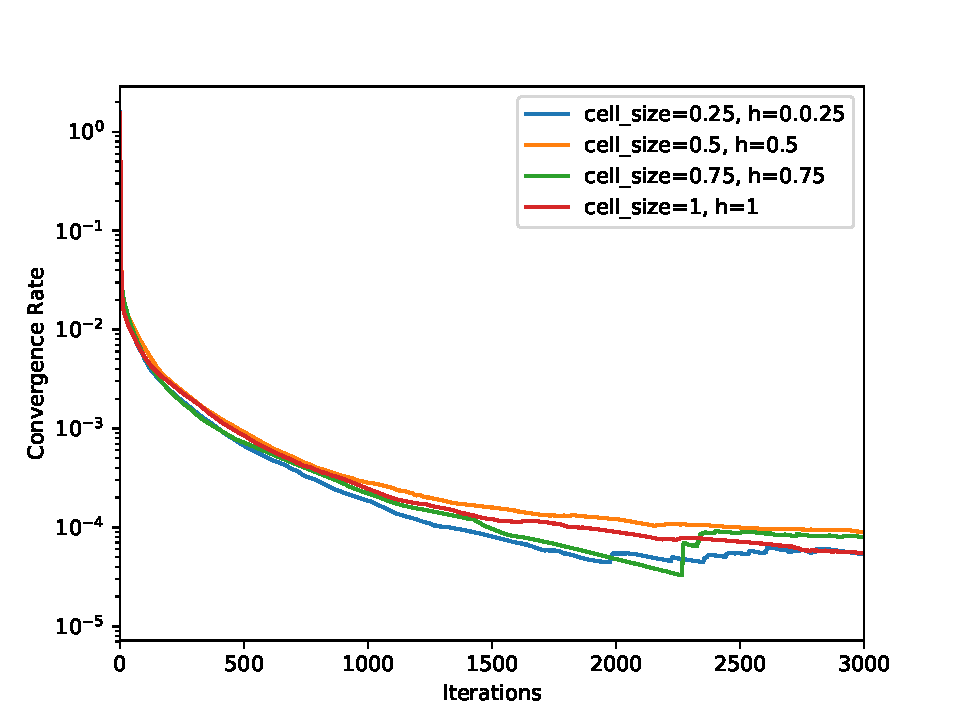
\includegraphics[width=\textwidth]{Figures/spikysize.pdf}
            \caption{Coveragence rate for different $d$ value.}
            \label{fig:spikyttime}
        \end{subfigure}
        \caption{Experiments for kernel \textbf{Spiky}.}
        \label{spiky}
    \end{figure}
    These two kernels are separately used based on Algorithm \ref{testsph}. In order to compare these two kernels carefully, the fixed iteration number was extended to $5000$. Then, the plot about the convergence rate of different kernels is obtained in Figure \ref{fig:testdkernel}. From the plot, it is clear that kernel \textbf{Poly6} perform better.  
    \begin{figure}[!ht]{}
        \centering
        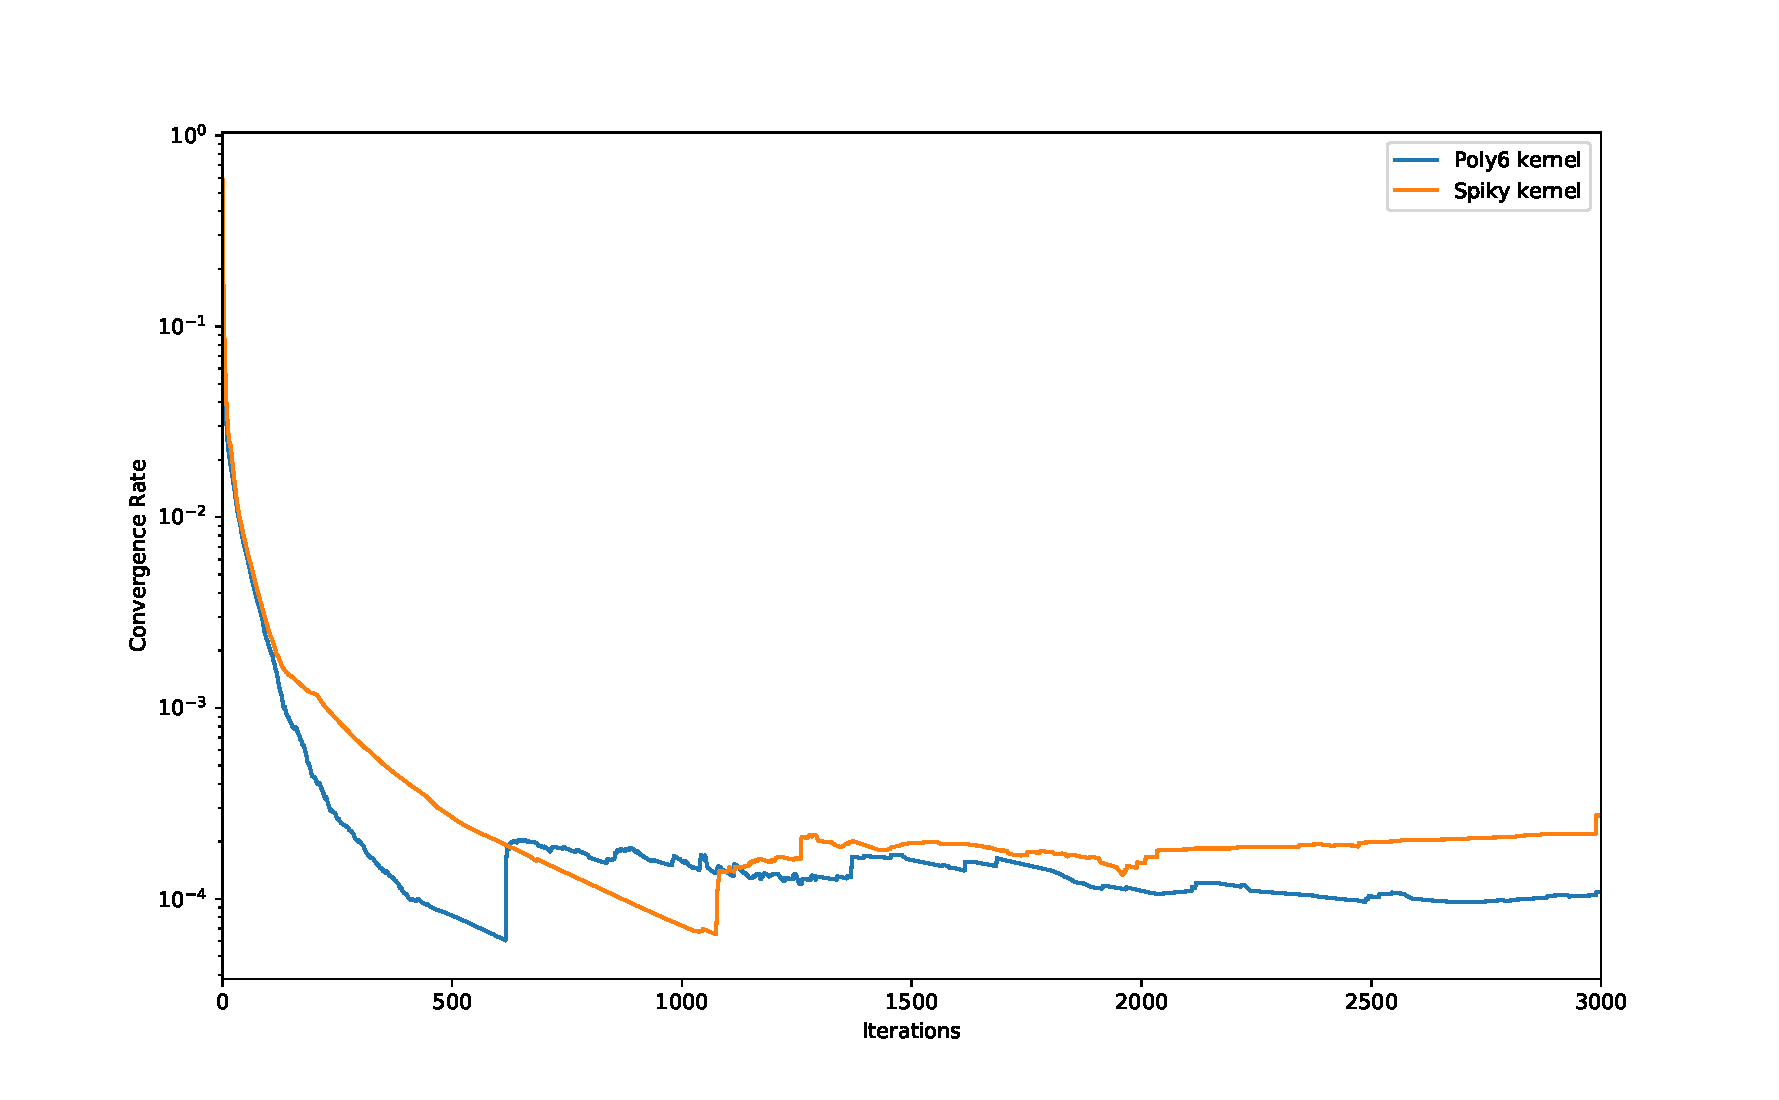
\includegraphics[width=0.8\textwidth]{Figures/kerneltest.pdf}
        \caption{Coveragence rate for kernel \textbf{Poly6} anf \textbf{Spiky}. $h_\text{poly6} = d_\text{poly6} = 0.5$, while $h_\text{spiky} = d_\text{spiky} = 0.25$}
        \label{fig:testdkernel}
    \end{figure}
    As a conclusion, SPH with \textbf{Poly6} kernel($\pmb{d} = (0.5, 0.5)$, smoothing length $h=0.5$), will be used for particle-grid transformation. \\

    After determining grid size and smoothing length, I will compare this specific \textbf{SPH-Model} with other models mentionde in section \ref{sphtest}, following Algorithm \ref{testsph}. The result is shown in Figure \ref{fig:final_test}.
     \begin{figure}[!ht]
        \centering
        \includegraphics[width=0.8\textwidth]{Figures/final_SPH.pdf}
        \caption{Coveragence rate for models(different initial values for $\pmb{\lambda}$).}
        \label{fig:final_test}
    \end{figure}
    Unlike the result shown in Figure \ref{fg:addsph}. Compared with other models, \textbf{SPH-Model} gets convergence much faster. So, $h=d=0.5$ is a good choice for this project and the future steps.

\section{Data Generation}
To create data that are more accessible to learning, I will map a discrete element method into a continuum setting use techniques from smooth particle hydrodynamics(SPH). In order to get enough available training data and remove useless information, I used,
\begin{itemize}
    \item Totally $150$ simulations with different initial configuration. The number of circle objects is not fixed as well. However, if there are too few objects inside the box, contacts might not happen until the simulation ends up. So the number of objects will be in the range of $[70, 110]$.
    \item If there is no contact in one state, the state means nothing to the learning. So the state files without any contacts will be removed.
\end{itemize}

\subsection{XML Restoration}
For each simulation, the state in every time step will be stored in one \textbf{XML} file. The structure of the body is consist of \textbf{mass}, \textbf{position}, \textbf{velocity}, \textbf{spin omega} and \textbf{inertia}. The structure of contact consists of \textbf{postion}, \textbf{impulse}(including in normal direction and tangent direcrion), \textbf{master} body and \textbf{slave} body. Two examples are given in the following.\\

This is an example of one body information is given below.
\begin{lstlisting}[language=XML]
    <body index="86" type="free">
        <mass value="3.14159274101"/>
        <position x="7.79289388657" y="2.62924313545"/>
        <velocity x="2.7878344059" y="-1.45545887947"/>
        <orientation theta="-0.115291565657"/>
        <inertia value="1.57079637051"/>
        <spin omega="-2.33787894249"/>
        <shape value="circle"/>
    </body>
    ...
\end{lstlisting}
Another example \textit{XML} code is for contatc force.
\begin{lstlisting}[language=XML]
    <contact index="1" master="2" master_shape="b2CircleShape(childCount=1, pos=b2Vec2(0,0), radius=1.2000000476837158, type=0,)" slave="97" slave_shape="b2CircleShape(childCount=1, pos=b2Vec2(0,0), radius=1.2000000476837158, type=0, )">
        <position x="0.21963849663734436" y="13.875240325927734"/>
        <normal normal="b2Vec2(-1,2.9819e-05)"/>
        <impulse n="0.005236322991549969" t="-0.002184529323130846"/>
    </contact>
    ...
\end{lstlisting}

\subsection{SPH configuration}
As it is talked in \ref{SPH-setting}, 
\begin{itemize}
    \item \textbf{Kernel}, Poly6, which you can see in section \ref{poly6}.
    \item \textbf{Kernel Settings}, cell size $d_x=d_y=0.5$, smoothing length $h=0.5$.
\end{itemize}
\subsection{XML to grid}
After getting a set of \textbf{XML} file, the next step is to load state information from \textbf{XML} file, and then map them to grid images with SPH based method. Since for any contact point, there are two normal contacts, one with $[n_x, n_y]$ while the other with $[-n_x, -n_y]$. So the grid values for $\pmb{n}$ would be always $\pmb{0}$, and the same  with $\pmb{t}$. So finally, the channel number of each image will be $6$, including $[m, v_x, v_y, \omega, \lambda_n, \lambda_t]$. \\

For the learning, I divide 8 channels into features(input) and label(output).
    $$\text{Feature} = [m, v_x, v_y, \omega]$$
    $$\text{Label} = [\lambda_n, \lambda_t]$$


\section{CNN Training}
\subsection{CNN  Architecture}
    The neural network was designed using Keras\cite{chollet2015keras}. Keras is a neural networks Application Programming Interface (API) written in Python, it runs on top of either TensorFlow. With some inspiration from AlexNet\cite{Krizhevsky:2012:ICD:2999134.2999257}, the networks shows five constructing stacks of layers and each stack is consist of two or three convolutional layers in the same size. To avoid overfitting, each stack is followed by one dropout layer. One full-connected layer is set after the last convolutional layer. This input layer is followed by a batch normalization layer, normalizing images within a batch, which is discussed in Section \ref{batchnor}. This architecture includes $51,599,092$ weights for an input size of ($61\times61\times4$). All convolutional layers have kernels of size $(3\times 3\times d)$, and are followed by ReLU activation function. Figure \ref{fig:art} shows the visualization of model architecture, and Table \ref{table:layers} shows the specific information about parameters when input images go through the CNN.
    \begin{itemize}
        \item \textbf{Input Size}, the input will be $61\times61\times4$. Since the orginal world is $30\times30$ and grid size is $d=0.5$, the generated grid would be $61\times61$. There would $4$ channels
        \item \textbf{Output Size}, output size depends on the label size. The orginal label image would be $[\lambda_n, \lambda_t]$, so the label image size would be $61\times61\times2$, which should be flattened as the actual training label. The label size would be $61\times 61 \times 2$
        \item \textbf{Weight Number}, the total weights number is $64,498,866$. 
    \end{itemize}

    \begin{figure}[!h]
        \centering
        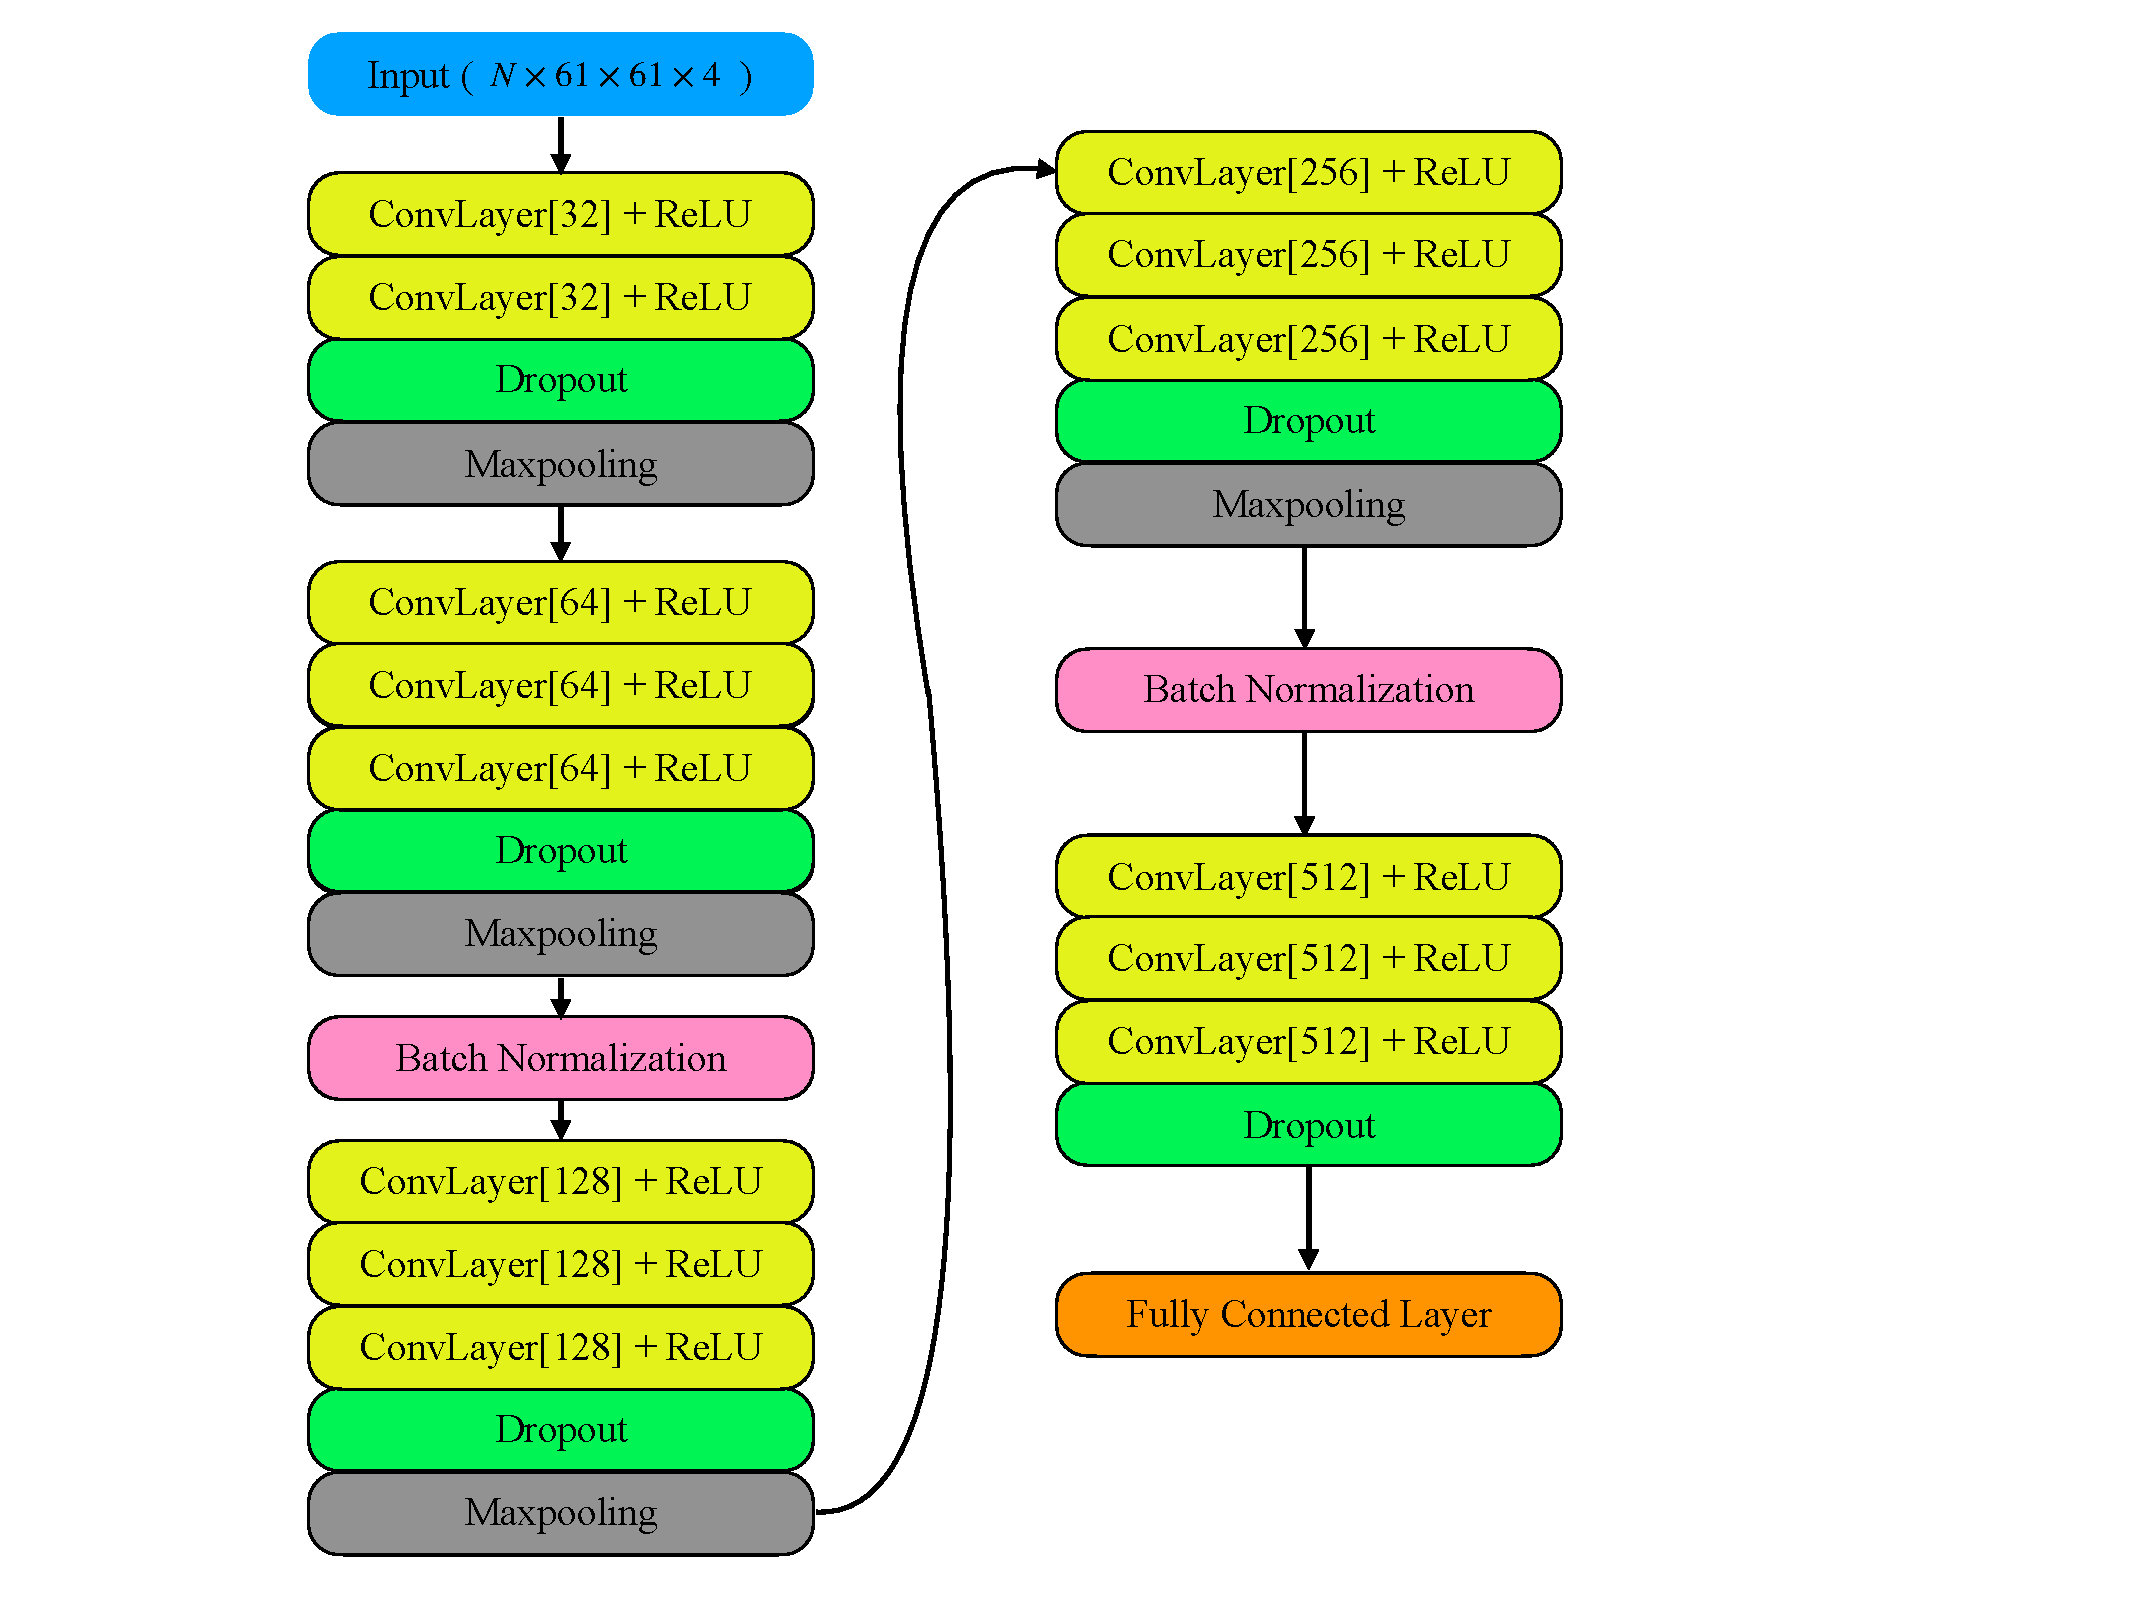
\includegraphics[width=\textwidth]{Figures/cnn_arc.pdf}
        \caption{Architecture of CNN model}
        \label{fig:art}
    \end{figure}

    \begin{table}[h!]
        \centering
        \begin{tabular}{ l | c  }
            Layer & Output Shape  \\ \hline
            Input & $n_b\times61\times61\times4$  \\
            Convolution(32) & $n_b\times61\times61\times32$  \\
            Convolution(32) & $n_b\times61\times61\times32$  \\
            Dropout & $n_b\times61\times61\times32$  \\
            MaxPooling & $n_b\times31\times31\times32$ \\
            Convolution(64) & $n_b\times31\times31\times64$  \\
            Convolution(64) & $n_b\times31\times31\times64$  \\
            Convolution(64) & $n_b\times31\times31\times64$  \\
            Dropout & $n_b\times31\times31\times64$  \\
            MaxPooling & $n_b\times16\times16\times64$ \\
            BatchNormalization & $n_b\times16\times16\times64$ \\
            Convolution(128) & $n_b\times16\times16\times128$  \\
            Convolution(128) & $n_b\times16\times16\times128$  \\
            Convolution(128) & $n_b\times16\times16\times128$  \\
            Dropout & $n_b\times16\times16\times128$  \\
            MaxPooling & $n_b\times8\times8\times128$ \\
            Convolution(256) & $n_b\times8\times8\times256$  \\
            Convolution(256) & $n_b\times8\times8\times256$  \\
            Convolution(256) & $n_b\times8\times8\times256$  \\
            Dropout & $n_b\times8\times8\times256$  \\
            MaxPooling & $n_b\times4\times4\times256$ \\
            BatchNormalization & $n_b\times4\times4\times512$  \\
            Convolution(512) & $n_b\times4\times4\times512$  \\
            Convolution(512) & $n_b\times4\times4\times512$  \\
            Convolution(512) & $n_b\times4\times4\times512$  \\
            Dropout & $n_b\times4\times4\times512$ \\
            Flatten & $n_b\times8192$ \\
            Dense & $n_b\times7442$ \\    
        \end{tabular}
        \caption{Feature map (tensor) sizes through the network, the input has size $n_b\times61\times61\times5$, with batch size $n_b$ and patches of size $61\times61\times5$.}
        \label{table:layers}
    \end{table}

\subsection{Traing Configuration}
\subsubsection{Loss Function}
Firstly, we define a filter funtion,
\begin{equation}
    g(x)= \begin{cases} 0, \quad x = 0 \\ 1, \quad x \ne 0 \end{cases}
\end{equation}
Then, we can update the loss function based on Euqation \ref{eq:mse}. 

\begin{equation}
    L = \frac{1}{N}\sum_{i}^{N}g(\hat{y}_i)(y_i-\hat{y}_i)^2
\end{equation}

\subsection{Training Details}
    The learning happened on GPU(\textit{GeForce GTX 1080 Ti, 11 Gbps GDDR5X memory})\footnote{\url{https://www.nvidia.com/en-us/geforce/products/10series/geforce-gtx-1080-ti/}} held by Image Section, DIKU\footnote{\url{https://di.ku.dk/english/research/imagesection/}}. The whole learning takes nearly 24 hours. The model you can download in my personal dropbox\footnote{\url{https://www.dropbox.com/s/jrwzqib6ghrq59i/model.h5?dl=0}}. I gave hyperparameters setting below,
    \begin{table}[h!]
        \centering
        \begin{tabular}{ l | c  }
            Hyperparameter  & Setting \\ \hline
            Activation function & ReLU \\
            Weight initilization & He normal\cite{sutskever2013importance} \\
            Weight regularizer &  L2 \cite{hinton2006fast} \\
            Convolution border mode  & Same \\
            Stride & 2 \\ 
            Kernel size & $(3, 3)$ \\
            Dropout rate & $0.1$ \\
            Optimizer & SGD \\
            Initial Learning Rate & $1\times 5\times10^{-3}$ \\
            Batch Size & 200 \\
            Epoch & 1000 \\
            Validation Rate & 0.2 \\
        \end{tabular}
        \caption{Hyperparameter settings.}
        \label{table:hyper}
    \end{table}
    \subsubsection{Learning Rate}
    The learning rate will change with the number of epoch, as talked in section \ref{learning}. I will give a specific value as the learning rate depending on the number of epoch. The learning rate will become smaller with increasing epoch. 
    data. The overall algorithm is concluded in Algorithm \ref{ls}.

    \subsubsection{Conclusion about Training process}
    \begin{itemize}
        \item The size of the input image is $41\times41\times4$, and all pixels are important since all of them retore useful information. If we want to extract the features from $41\times 41$, $3\times 3$ kernel would be a good choice. But the disadvantages is that there would be a lot of training parameters, which might slow down the learning process.
        \item I do have nearly $18208$ samples for training. However, it is hard for both the GPU and CPU to load all the data at one time. Dividing all training samples to a couple of batches would not only speed up the single training time and release memory, but also reduce the risk of overfitting.
        \item The learning rate will change with the number of the epoch, as analyzed in section \ref{learning}. I will give a specific learning rate values depending on the number of the epoch. The learning rate will become smaller with With the epoch increase, I hope the value of learning rate can decrease. Since the high learning rate would cause suboptimal performance at the end of training. The overall algorithm is concluded in Algorithm \ref{ls}.
        \item Validation data set is essential to test the accuracy of the model and whether it is overfitting. Before each epoch, validation would be randomly selected, $20\%$ of total data.
    \end{itemize}

    \begin{algorithm}[!h]
        \KwData{$epoch$}
        \KwResult{learning rate $\eta$}
        \If {$epoch < 100$}{$\eta = 5\times10{-3}$}
        \If {$100< epoch < 300$}{$\eta = 2\times10^{-3}$}
        \If {$300< epoch < 500$}{$\eta = 1\times10^{-3}$}
        \If {$epoch > 300$}{$\eta = 2\times10^{-4}$}
        \caption{Learning Rate Scheduling}
        \label{ls}
    \end{algorithm}


\section{Simualtion based on Trained Model}
Once getting the trained model, the next step is to apply this model in simulation based on Algorithm \ref{al:basic} and compare it with other solutions. The details of process is described in Algorithm \ref{al:basic}
\begin{figure}[!h]
    \centering
    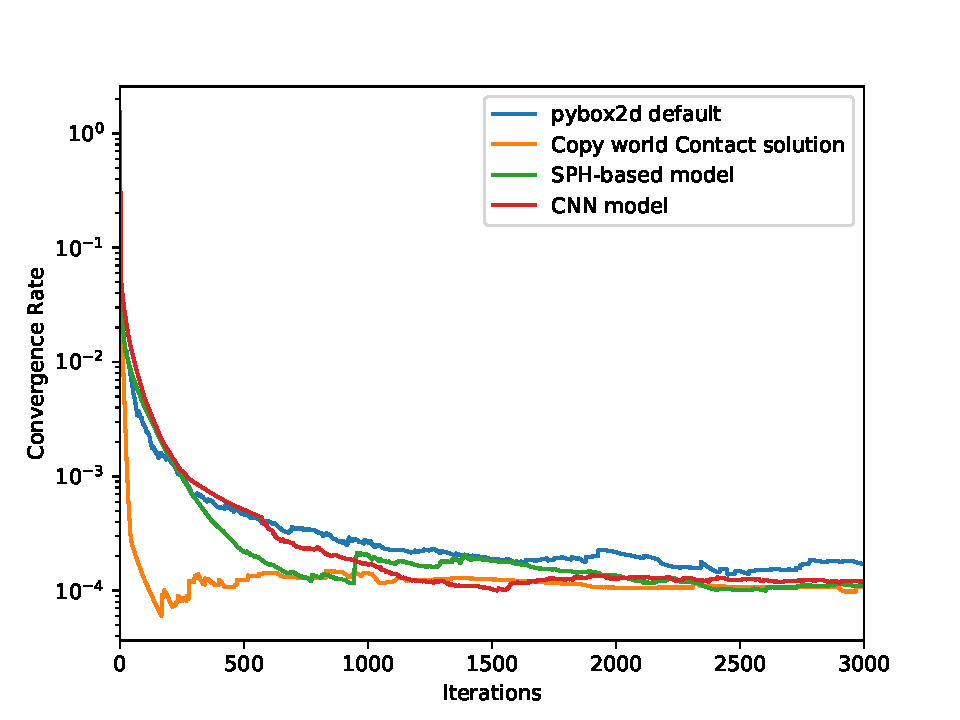
\includegraphics[width=0.8\textwidth]{Figures/same_world.pdf}
    \caption{The final result. Add the final CNN solution to compare with other methods.}
    \label{testoneworld}
\end{figure}

I applied it in one test world built by the setting mentioned in section \ref{simconfig}. The test world is consist one $30 \times 30 $ box and $K$($50<K<100$) randomly distributing balls($r=1$). The balls will fall down due to gravity. Figure \ref{testoneworld} shows the details. As what is expected, CNN model performs similar with \textbf{SPH-Model}(mentioned in section \ref{sphtest}). Although the model is not as good as \textbf{SPH-model}, its coverages rate is obviously faster than built-in ones. 
From Figure \ref{testoneworld}, it can be indicated that the CNN model actually makes the iterative solver converge faster. But it is just a small improvement. The CNN solution cannot reach a convergence as rapidly as \textbf{Copy-Model}. It is mainly the limitation of the SPH-based method. When the particle .

\begin{algorithm}[!h]
        \KwData{
            Given a set of bodies $\mathcal{B}$ and the state in time $t$, as well as some information of contacts between these bodies $\mathcal{C}$.
        }
        \KwResult{Get the contact forces $\pmb{\lambda}_{j}=[{\lambda_{n}}_{j}, {\lambda_{t}}_j]~~j\in\mathcal{C}$ at time $t$.}
        \While{Simulation Runing}
        {
            1. read the current state, $\mathbf{x}=(x_i, y_i)$ is the spatial position of one node in the grid image.
                $$m_i, \pmb{v}_i, \pmb{q}_i, \omega_{i}~~i\in\mathcal{B}$$
                $$\pmb{n}_j~~j\in\mathcal{C}$$ \\
            2. map the current state to a gird image,
                $$G_{m}(\mathbf{x}) \equiv \sum_{i\in \mathcal{B}}W(\mathbf{x}, \pmb{q}_{i})m_i$$ 
                $$G_{\pmb{v}}(\mathbf{x}) \equiv \sum_{i\in \mathcal{B}}W(\mathbf{x}, \pmb{q}_{i})\pmb{v}_i,~~\pmb{v}=(v_x, v_y)$$
                $$G(\mathbf{x}) = [G_{m}(\mathbf{x}), G_{\pmb{v}}(\mathbf{x}), G_{\pmb{n}}(\mathbf{x})]$$ \\
            3. Use $G(\mathbf{x})$ as the input image to the learning model, the output will be resize to a imag, the output image will be called $G_{output}$,
                $$G_{output}(\mathbf{x}) = [G_{\lambda_{n}}(\mathbf{x}), G_{{\lambda}_{t}}(\mathbf{x})]$$ \\
            4. Once the contact force image is obtained,  the conatct position $\pmb{q}_{j} = (x_{j}, y_{j})~~j\in\mathcal{C}$  will be used to interpolation image values based on Equation \ref{interpolation}.
                $$\pmb{\lambda}_j \approx G_{output}(\pmb{q}_j)~~j\in\mathcal{C}$$ 
            The interpolated values $\pmb{\lambda}$ will be used as starting iterated for \textit{pybox2d} conatc solver to find a final solution. \\
            5. Update $t$
                $$t = t + \Delta t$$ \\
        }
        \caption{Introducrion to the deep contact model solver in this thesis.}
        \label{al:basic}
\end{algorithm}
